\documentclass[11pt]{article}
\usepackage{charter}
\usepackage{graphicx}
\usepackage{hyperref}
\usepackage{mdframed}
\usepackage[margin=1in]{geometry}
\usepackage{amsmath}

\hypersetup{
	colorlinks=true,
	linkcolor=blue,
	filecolor=magenta,
	urlcolor=cyan,
}

\begin{document}

%===================================================
% Title and Author Info
%===================================================
\begin{center}
{\Large\textsc{Relativistic Orbits}} \\
\vspace{10pt}
{\large \textbf{Mentor:} Alex Urban} \\
{\small LIGO Laboratory, California Institute of Technology \\
Pasadena, CA 91125, USA \\
\href{mailto:aurban@ligo.caltech.edu}{\texttt{aurban@ligo.caltech.edu}}}
\end{center}

%%%%%%%%%%%%%%%%%%%%%%%%%%%%%%%%%%%%%%%%%%%%%%%%%%%

\section*{Purpose}

\hspace{15pt} In this problem set, we will try out a better numerical integration scheme, then work out the total energy of a ``simple'' relativistic orbit and simulate it in Python. We will also look at a fun toy problem that starts to get at the dynamics that lead to electromagnetic counterparts of compact binary mergers. The goal is to start putting together all the astrophysics we've been learning in an awesome relativistic orbit simulation.... \textit{of science!}

\section*{Relativistic Orbits in a Simple Curved Spacetime}
\hspace{15pt} Suppose that a neutron star binary (each with mass $M = 1.4\,\, M_{\odot}$) is in a stable orbit, still with no loss of energy, but now in Schwarzschild spacetime. Figure \ref{fig:binary_diagram} illustrates this system.

\vspace{20pt}

\begin{figure}[!h]
\begin{mdframed}
\centering
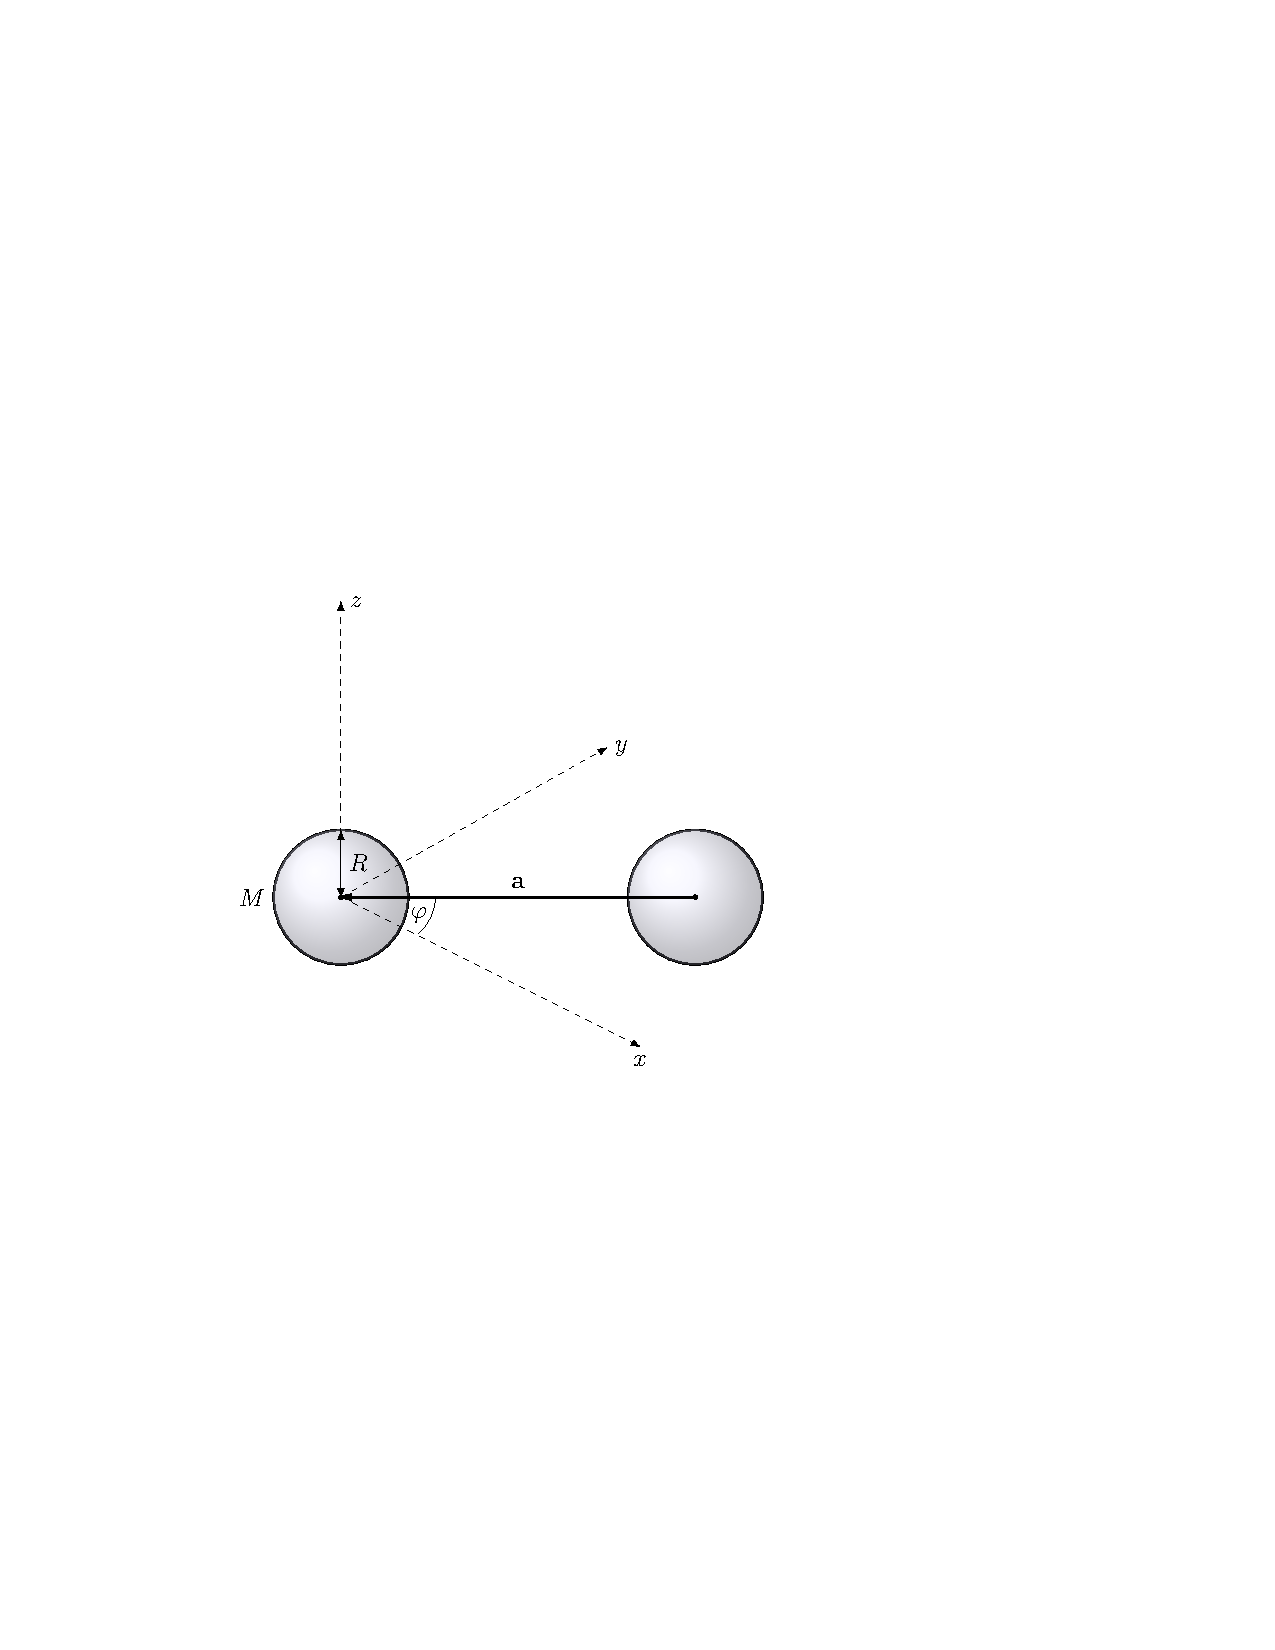
\includegraphics{relativistic_orbit/binary_diagram.pdf}
\caption{\label{fig:binary_diagram}Diagram of the neutron star binary in the center of mass frame, showing its orbital separation vector ($\mathbf{r}$) and the radius ($R$) and masses ($m_1$, $m_2$) of the individual neutron stars. The azimuthal angle $\varphi$ is also indicated.}
\end{mdframed}
\end{figure}

\vspace{1000pt}

\begin{enumerate}

\item First, we want to experiment with a better numerical integrator using a problem we already understand. Try re-doing the Keplerian orbit simulation, only this time, use the RK4 integration scheme: if $t_i, \dots, t_N$ are a series of time samples and $df/dt = g(f, t)$ a differential equation for some set of functions $f$, then the RK4 method
\begin{align*}
k_1 &= g(f(t_i), \, t_i) \\
k_2 &= g\left(f(t_i) + \frac{k_1}{2}\Delta t, \, t_i + \frac{1}{2}\Delta t\right) \\
k_3 &= g\left(f(t_i) + \frac{k_2}{2}\Delta t, \, t_i + \frac{1}{2}\Delta t\right) \\
k_4 &= g(f(t_i) + k_3\,\Delta t, \, t_i + \Delta t) \\
f(t_{i+1}) &= f(t_i) + \frac{\Delta t}{6}\,\left(k_1 + 2k_2 + 2k_3 + k_4\right)
\end{align*}
is a generalization of Simpson's rule with step size $\Delta t$.

\hspace{15pt} Show that, for the Keplerian orbit problem, the RK4 method still conserves energy and angular momentum, and that it allows you to use a much larger step size without introducing numerical error. (How much larger can the step size be?)

\item To visualize some important effects from general relativity, consider a correction to the total energy that comes from the simplest example of curved spacetime:
\begin{equation}
\frac{1}{2} \left(\frac{E^2}{\mu c^2} - \mu c^2\right) = \frac{1}{2}\mu\left(\frac{dr}{d\tau}\right)^2 + \Phi(r, L)
\end{equation}
where $\tau$ is the proper time, $\mu = m_1 m_2/(m_1 + m_2)$ is the reduced mass, $M = m_1 + m_2$ is the total mass, and the effective potential
\begin{equation}\label{eq:potential}
\Phi(r, L) = -\frac{GM\mu}{r} + \frac{L^2}{2\mu r^2} - \frac{GML^2}{c^2\mu r^3}
\end{equation}
now has an extra attractive centrifugal term. Using what you know about calculus and circular orbits, show that with this potential there can be no stable circular orbits closer than a radius
\begin{equation}\label{eq:ISCO}
r_{\rm ISCO} = \frac{6GM}{c^2}.
\end{equation}
In astrophysics jargon, this is called the ISCO radius (short for Innermost Stable Circular Orbit). At what gravitational wave frequency does ISCO occur?

\item Perform a simulation of orbits in this spacetime, using masses of 1.4 $M_{\odot}$ for each body and experimenting with different initial conditions. What angular momenta do you need to visualize ISCO properties? If you use RK4, is the total (relativistic) energy conserved?

\item Finally, let's have some fun with a toy problem that works as a surprisingly good model for the physics of $\gamma$-ray bursts: the relativistic cannonball. Suppose a cannonball of mass $m_1$ moving at Lorentz factor $\Gamma$ collides with another particle of mass $m_2$ that is initially at rest.
\begin{enumerate}
\item To a very distant observer watching this epic lightshow (at rest), what is the time between the muzzle flash of the cannon and the collision of the masses? Write this in terms of the time as measured in the rest frame of $m_1$.

\item If the collision is completely inelastic (so that the masses stick together), use the conservation of 4-momentum to find the final energy and momentum, and write the final Lorentz factor in terms of the mass ratio $m_1/m_2$.
\end{enumerate}

\end{enumerate}

%%%%%%%%%%%%%%%%%%%%%%%%%%%%%%%%%%%%%%%%%%%%%%%%%%%

\section*{Things That Make You Go, ``Hmmm....''}

\begin{enumerate}

\item How much energy is available at the ISCO radius to power gravitational radiation and $\gamma$-ray bursts?

\item What does your figure for $m_1/m_2$ in the last problem tell us about the mass of the disk that forms during compact binary mergers? Full disclosure: this is not a trick question, but it's also not an easy one. There is a lot of physics that goes into answering this, but I want you to try mulling it over. Don't be afraid to use tools like google; in fact, doing a literature search is generally always a great thing to do when you want to understand something new!

\item Suppose we add to the Keplerian system a tiny point particle of mass $m \ll M$. What do you think its motion would look like in different regions?

\end{enumerate}

%%%%%%%%%%%%%%%%%%%%%%%%%%%%%%%%%%%%%%%%%%%%%%%%%%%

\vspace{1000pt}

%%%%%%%%%%%%%%%%%%%%%%%%%%%%%%%%%%%%%%%%%%%%%%%%%%%

\subsection*{Solution}

\begin{enumerate}

\item 

\item In classical mechanics, the two-body problem can be solved exactly in terms of an ``equivalent one-body'' situation, where a particle of mass $\mu = m_1 m_2/(m_1 + m_2)$ behaves as though it's interacting with a stationary particle of mass $M = m_1 + m_2$. There \emph{is} a version of this in general relativity, but it's absurdly complicated (see, for example, \href{https://arxiv.org/pdf/gr-qc/9811091.pdf}{arXiv pre-print gr-qc/9811091}). What I'm giving you here is a first-order approximation that isn't complete, but does capture most of the interesting physics. Once again, we'll think in terms of the center of mass.

\hspace{15pt} In Newtonian terms, the effective potential in Eq. \ref{eq:potential} results in a central, conservative force
\begin{equation}\label{eq:schswarzschild_force}
\mathbf{F}(r; L) = -\frac{\partial\Phi}{\partial r}\,\hat{\mathbf{r}} = \left( -\frac{GM\mu}{r^2} + \frac{L^2}{\mu r^3} - \frac{3GML^2}{c^2\mu r^4} \right) \, \hat{\mathbf{r}}.
\end{equation}
This isn't really a force at all -- it's a constraint that defines \textit{timelike geodesics}, or shortest paths through curved spacetime. The acceleration felt as a result of this ``force'' is called a \textit{proper acceleration}, and it is measured as a function of the proper time $\tau$ of the moving star.

\hspace{15pt} The extra centrifugal term in Eq. \ref{eq:schswarzschild_force} represents an extra attraction that is purely relativistic. In a cartoon-y way, we can think of it as some extra kinetic energy delivered onto moving objects by the curved spacetime they're passing through. Stable circular orbits will occur wherever the gravitational and centrifugal forces are balanced, or
\[ F(r; L) = -\frac{GM\mu}{r^2} + \frac{L^2}{\mu r^3} - \frac{3GML^2}{c^2\mu r^4} = 0. \]
This occurs at certain radii given by
\begin{equation}\label{eq:circ}
r_{\rm C} = \frac{h^2 \pm \sqrt{h^4 - 12h^2G^2M^2/c^2}}{2GM}
\end{equation}
where $\mathbf{h} = \mathbf{L}/\mu$ is the orbital angular momentum per unit mass (see Figure \ref{fig:schwarzschild_potentials}).

\hspace{15pt} Note from Eq. \ref{eq:circ} that there can now be \emph{two} places where the forces are balanced. The larger of these is a local minimum of $\Phi$ -- the stable circular orbit we're familiar with. The smaller radius will be an unstable circular orbit, caused by the extra $L^2/r^4$ centrifugal force. And that's not even all -- note further that if the angular momentum is too small, then what's under the square root in Eq. \ref{eq:circ} will be negative, meaning we can only get stable circular orbits when
\begin{equation}
\frac{L^2}{\mu^2} \geq \frac{12G^2M^2}{c^2}.
\end{equation}
The innermost stable circular orbit will occur when these terms are equal, at which point the orbit has a radius
\begin{equation}
r_{\rm ISCO} = \frac{6GM}{c^2}
\end{equation}
(see Fig. \ref{fig:schwarzschild_potentials}). Because these relativistic orbits still satisfy Kepler's third law, we know that at this radius the system will be emitting gravitational waves at a frequency
\[ f_{\rm ISCO} = \frac{1}{\sqrt{216\pi^2}} \frac{c^3}{GM}. \]
Thus, binaries with higher total mass will merge at lower frequencies. (For a non-spinning neutron star binary where each body has a mass 1.4 M$_{\odot}$, we predict the ISCO frequency is around 2800 Hz.)

\hspace{15pt} The ISCO radius is very important. In relativistic orbits, it effectively tells us when two compact objects are about to merge. It is the point past which all orbits that lose any energy can't help but quickly spiral inward. A conceptually neat and very important question is: how much energy has been given off by this point? If we think of the total energy $E=k\mu c^2$ as a fraction of the rest mass-energy (which can happen because the potential is negative), then from Eq. \ref{eq:potential} we can estimate the fraction $k$ of rest mass left over by the time the neutron stars reach ISCO:
\[ c^2(k^2 - 1) = \frac{2\Phi_{\rm ISCO}}{\mu} = -\frac{2GM}{r_{\rm ISCO}} + \frac{L_{\rm ISCO}^2}{\mu^2 r_{\rm ISCO}^2} - \frac{2GML_{\rm ISCO}^2}{c^2\mu^2r_{\rm ISCO}^3} = -\frac{c^2}{9}. \]
Put another way, this means roughly $1-k \simeq$ 5.7\% of the rest mass was lost! If $\mu \sim$ 1 M$_{\odot}$, that's upwards of 10$^{46}$ J of energy --  where did it all go? This question will drive the next part of our investigation.

\begin{figure}[!t]
\centering
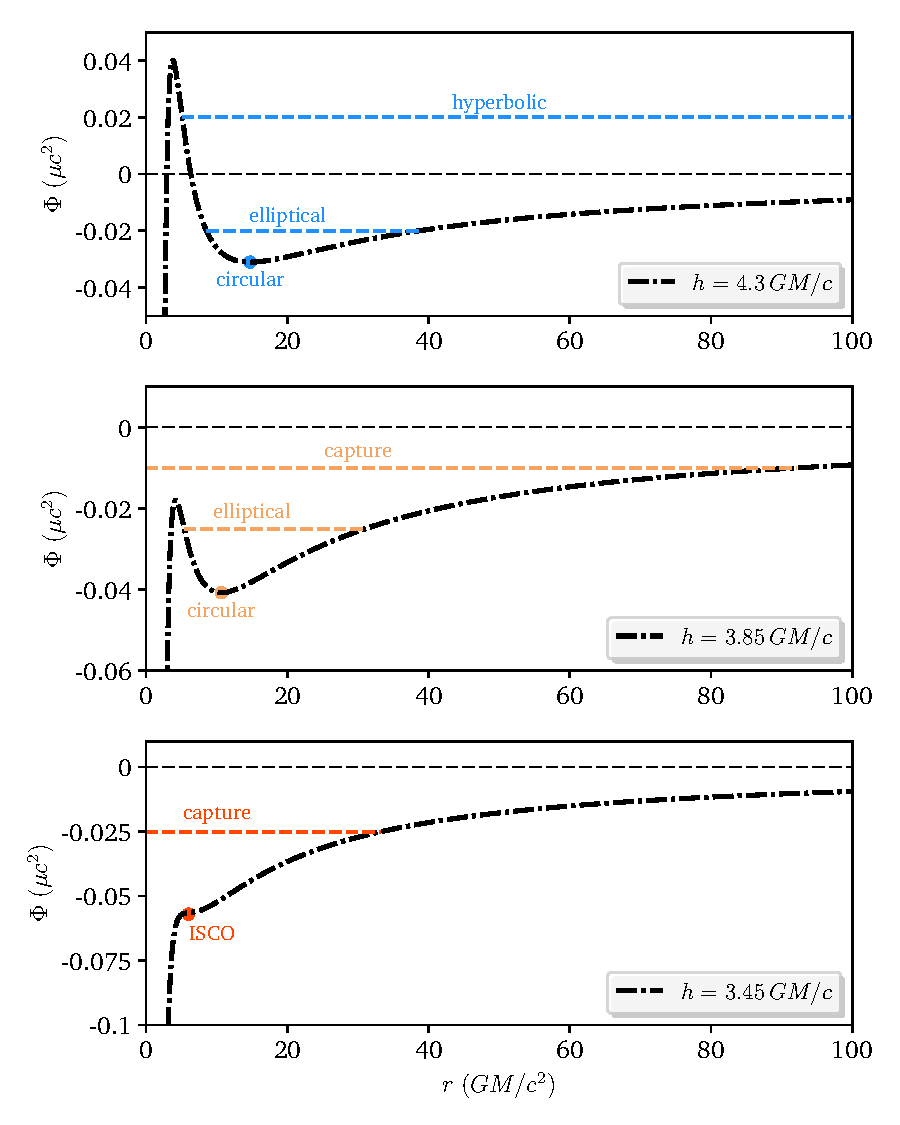
\includegraphics{relativistic_orbit/schwarzschild_potentials.pdf}
\caption{\label{fig:schwarzschild_potentials}Visualization of effective potentials in curved spacetime, with different snapshots of the angular momentum per unit mass $\mathbf{h} = \mathbf{L}/\mu$. Top: a large value of $h$ leads to the centrifugal barrier we're used to seeing at small $r$. In this case, there are both bound (elliptical) and unbound (hyperbolic) orbits. Middle: A smaller angular momentum weakens the centrifugal barrier, leading to so-called ``capture orbits'' where the extra kinetic energy causes one body to careen into the other. Bottom: The smallest angular momentum possible that still has a stable circular orbit (the ISCO). All other orbits in this potential (and those with smaller $h$) are capture orbits.}
\end{figure}

\item 

\item 

\end{enumerate}

%%%%%%%%%%%%%%%%%%%%%%%%%%%%%%%%%%%%%%%%%%%%%%%%%%%

\begin{mdframed}

\section*{Things That Make You Go, ``Hmmm....''}

\begin{enumerate}

\item How much energy is available at the ISCO radius to power gravitational radiation and $\gamma$-ray bursts?

\item What does your figure for $m_1/m_2$ in the last problem tell us about the mass of the disk that forms during compact binary mergers? Full disclosure: this is not a trick question, but it's also not an easy one. There is a lot of physics that goes into answering this, but I want you to try mulling it over. Don't be afraid to use tools like google; in fact, doing a literature search is generally always a great thing to do when you want to understand something new!

\item Suppose we add to the Keplerian system a tiny point particle of mass $m \ll M$. What do you think its motion would look like in different regions?

\end{enumerate}

\end{mdframed}

\end{document}
